\documentclass[UTF8,a4paper]{ctexart}%设置a4纸和中文
\ctexset{section/format=\Large\bfseries}%设置标题左对齐
\usepackage{amsmath} % 使用align
\usepackage[margin=1in]{geometry}%设置A4值的边界
\usepackage{graphicx}%插入图片
\author{qhy}%作者
\date{\today}%日期
\title{计算机组成}%标题
\pagestyle{empty}%不显示页码
\begin{document}
  \maketitle
  \tableofcontents
  \newpage
  \section{虚拟存储器}
      \subsection{基本概念}
          \begin{itemize}
            \item 虚拟存储器

            指一个容量非常大的存储器的逻辑模型,借助于磁盘等辅助来扩大主存容量,是指"主存-外存"这一存储层次。

            \item 基本特征

            虚拟空间大于实存空间,虚拟空间由辅存支持。

            \item 虚拟存储器和Cache的比较
                \begin{itemize}
                  \item Cache和主存交换数据的频率比较高,而虚存和主存交换数据的频率比较低。

                  \item Cache是提高存储系统的访问速度,它的所有功能由硬件实现。虚存解决的是存储系统的容量,它的所有功能是由操作系统通过软件和硬件来实现的。

                  \item Cache块的大小是固定的,每块的内容也比较小。虚存每次交换的量比较大。
                \end{itemize}
            \item 三级存储体系(见图\ref{fig1})
                \begin{figure}[!htp]
                  \centering
                  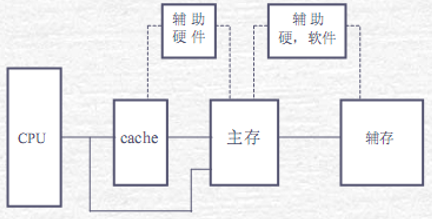
\includegraphics[scale=0.8]{assets/jisuanjizucheng2_14007.png}
                  \caption{三级存储体系}
                  \label{fig1}
                \end{figure}
                
                在三级存储体系中,\emph{Cache-主存}和\emph{主存-辅存}这两个存储层次的相同点:
                \begin{itemize}
                  \item 出发点相同

                      两者都是为了提高存储系统的性能价格比而构造的层次存储体系,都力图使存储系统的性能接近高速存储器,而价格接近低速存储器

                  \item 原理相同

                      都是利用程序运行时的局部性原理,把最近常用的信息快从相对慢速而大容量的存储器中调入相对高度而小容量的存储器中。
                \end{itemize}

                两者的不同点:
                \begin{itemize}
                  \item 目的不同

                      Cache主要解决主存与CPU的速度差异问题,而虚存就性能价格比的提高而言,主要解决存储容量的问题(另外还包括存储管理、主存分配和存储保护等方面)

                  \item 数据通路不同

                      CPU与Cache和主存之间均由直接访问的通路,Cache不命中时可直接访问主存,而虚存的辅存与CPU之间不存在直接的数据通路,当主存不命中时,只能通过调页解决,CPU最终还是要访问主存。

                  \item 透明性不同

                      Cache的管理完全由硬件完成,对系统程序和应用程序均透明,而虚存管理由软件(操作系统)和硬件共同完成,对系统程序不透明,对应用程序透明(段氏和段页式管理对应用程序"半透明")

                  \item 未命中时的损失不同

                      由于主存的存取时间是Cache的5~10倍,而辅存的存取时间通常是主存的存取时间的上千倍,故虚存未命中时系统的性能损失远大于Cache未命中时的损失。
                \end{itemize}

            \item 几个术语
                \begin{itemize}
                  \item 逻辑地址(虚地址):虚拟程序所提供的地址(是程序的逻辑地址)。

                  \item 虚拟地址空间:程序的逻辑地址空间。

                  \item 物理地址(实地址):CPU用于访问主存的地址。

                  \item 物理地址空间:物理地址所包含的存储空间。

                  \item 程序的再定位:程序进行虚地址到实地址的转换过程。
                \end{itemize}
          \end{itemize}
      \subsection{管理方式}
          \begin{itemize}
            \item 段式管理

                程序按逻辑结构分段,主存按段来分配存储管理方式。


                优缺点:
                \begin{itemize}
                  \item 优点

                      \begin{itemize}
                        \item 段的分界与程序的自然分界相对应
                        \item 段的逻辑独立性使得它易于编译、管理、修改和保护,也便于多道程序共享。
                        \item 某些类型的段(堆栈,队列)具有动态可变长度,允许自由调度以便有效利用空间。

                      \end{itemize}

                  \item 缺点

                      段间的零碎空间(碎片)不好利用。

                \end{itemize}
          \end{itemize}
      \subsection{工作过程}
\end{document}
